\section{Panorama energetico attuale}
La \textit{rete elettrica} attuale è il risultato di una rapida urbanizzazione e di un rapido sviluppo di infrastrutture in varie zone del mondo. Sebbene tali reti esistano ormai in molte aree geografiche diverse, le aziende generalmente tendono ad adottare tecnologie molto simili tra di loro. Ciononostante, restano altri fattori  di varia natura (economica, politica, geografica) legati allo sviluppo energetico che si diversificano a seconda dell'azienda. \newline
In generale però, pur tenendo in considerazione le differenze portate da tali fattori, la topologia base della rete elettrica attuale è rimasta immutata.
\begin{figure}[h] \centering{
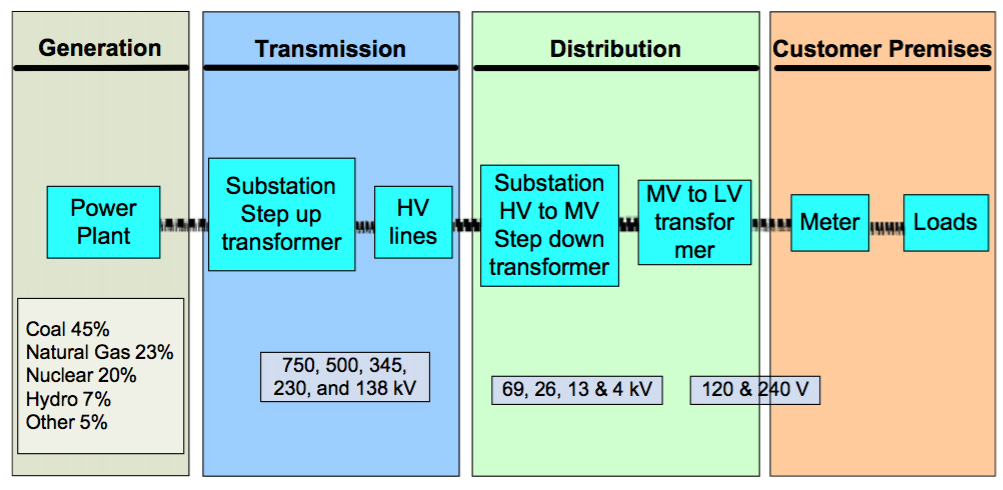
\includegraphics[scale=0.3, natwidth=1003,natheight=490]{imgs/elect_grid.png}}
\caption{La rete elettrica attuale}
\end{figure}
\newline La struttura della rete attuale è una struttura strettamente gerarchica. La figura 1.1 mostra l'esistenza di tre sottosistemi distinti: generazione, trasmissione e distribuzione. \newline Le centrali elettriche sono composte da generatori elettromeccanici i quali, durante la fase di \textbf{generazione}, spinti dal flusso dell'acqua corrente o da motori termici alimentati da combustioni chimiche, generano energia. Tale energia viene successivamente inviata ai trasformatori del livello di \textbf{trasmissione}, i quali la convertiranno in energia ad alto voltaggio per permetterne la diffusione a lunga distanza. Dopo tale step, si passa alla \textbf{distribuzione}, in cui si applica prima una trasformazione a medio e basso voltaggio e, in seguito, si procede all'erogazione agli utenti finali.
\newline Tale sistema è basato sostanzialmente su una comunicazione \textit{unidirezionale} in cui la sorgente non ha nessuna informazione real-time circa le necessità degli ultimi punti della catena. Pertanto si tende a sovraccaricare la rete, facendole raggiungere a priori i picchi massimi di carico; poiché è raro che le richieste degli utenti raggiungano tali valori, questo approccio porta a rendere la rete elettrica un meccanismo inefficiente.
\newline
Inoltre, le reti elettriche attuali sono interconnesse tra loro a formare reti regionali o nazionali con lo scopo di fornire rotte ridondanti e alternative per il flusso della corrente in caso di problemi. \newline
La distribuzione dell'energia è gestita da un \textit{controllore centralizzato} che ha il compito di amministrare diverse regioni da un'unica posizione centrale. 
\newpage
\section{Cenni storici}
Le tecnologie connesse con le reti elettriche hanno radici che risalgono alla fine del XIX secolo: la \textit{corrente diretta} di Thomas Edison e la \textit{corrente alternata} di Nikola Tesla continuano ad essere utilizzate tutt'ora. Oggi, infatti, l'energia viene trasmessa utilizzando la corrente alternata, mentre quella diretta ha applicazioni specifiche, solitamente all'interno di plessi residenziali e commerciali. \newline \newline
Le principali topologie di rete elettrica attualmente in uso sono due: \textbf{radial grid} e \textbf{mesh grid}.


\begin{figure}[h]\centering{
  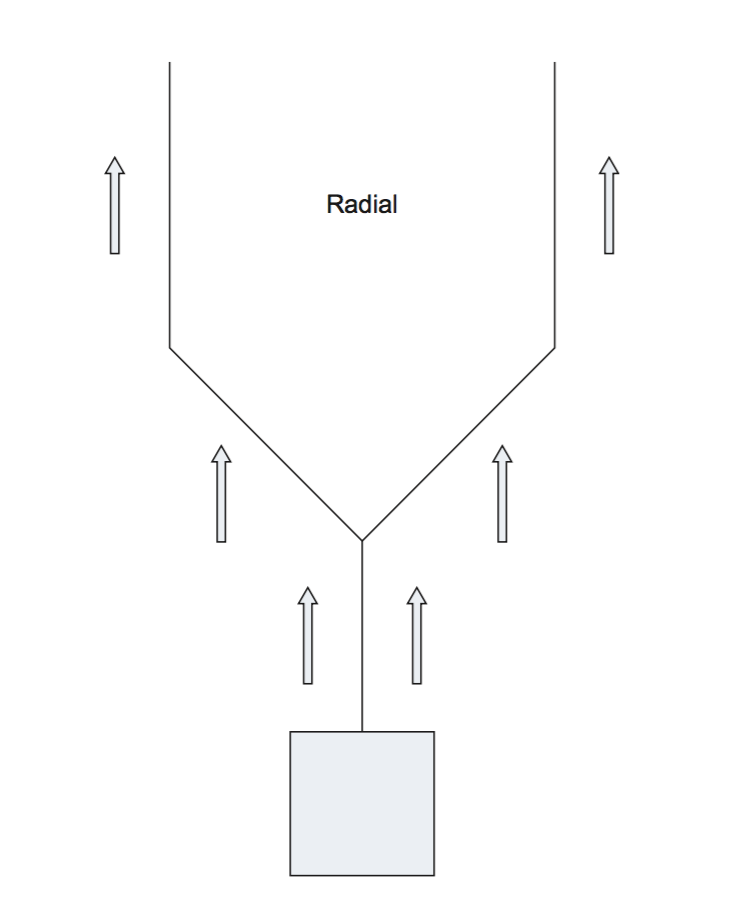
\includegraphics[scale=0.2, natwidth=754,natheight=909]{imgs/radialgrid.png}
  \caption{Radial grid}
}
\end{figure}

La radial grid (figura 1.2) è la topologia più comune; in essa l'elettricità viene distribuita a partire da una sottostazione seguendo un modello che ricorda un albero con molti rami e foglie.
Man mano che l'energia fluisce attraverso i cavi elettrici, la sua forza viene ridotta finchè non raggiunge la destinazione.

\begin{figure}[h]\centering{
  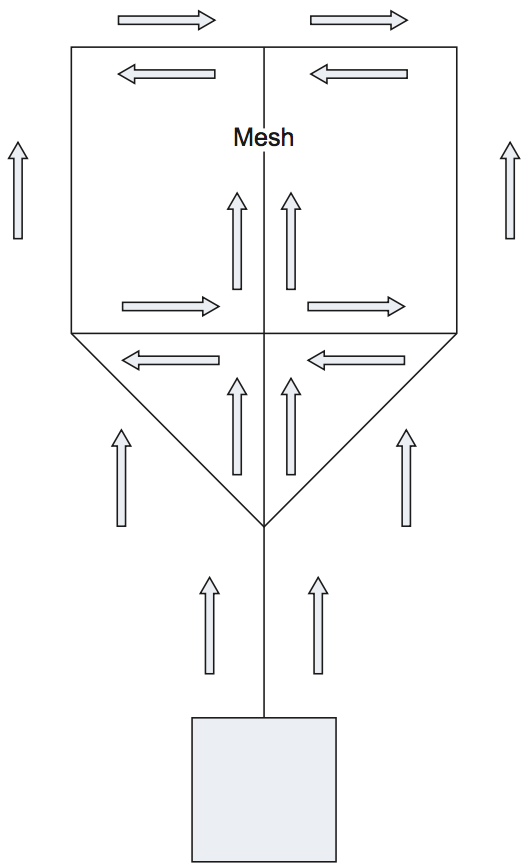
\includegraphics[scale=0.2, natwidth=529,natheight=867]{imgs/meshgrid.png}
  \caption{Mesh grid}
}
\end{figure}

La mesh grid (figura 1.3) fornisce una maggiore affidabilità rispetto alla radial grid poichè in quest'ultima ogni ramo ed ogni foglia ricevono energia da una singola sorgente (l'albero), mentre in una mesh l'energia può essere fornita attraverso varie fonti (altri rami e foglie). \newline
Le radial grid forniscono, inoltre, ridondanza limitata: in caso di malfunzionamento, una sottostazione vicina può entrare a far parte della rete, ma ciò presuppone che tale sottostazione non sia nelle stesse condizioni di quella che ha generato il guasto. \newline
Queste due topologie sono molto diffuse negli Stati Uniti.
Vi è, poi, una terza topologia utilizzata principalmente in Europa: \textbf{looped topology}, nata come insieme delle due reti precedenti (figura 1.4). 

\begin{figure}[h]\centering{
  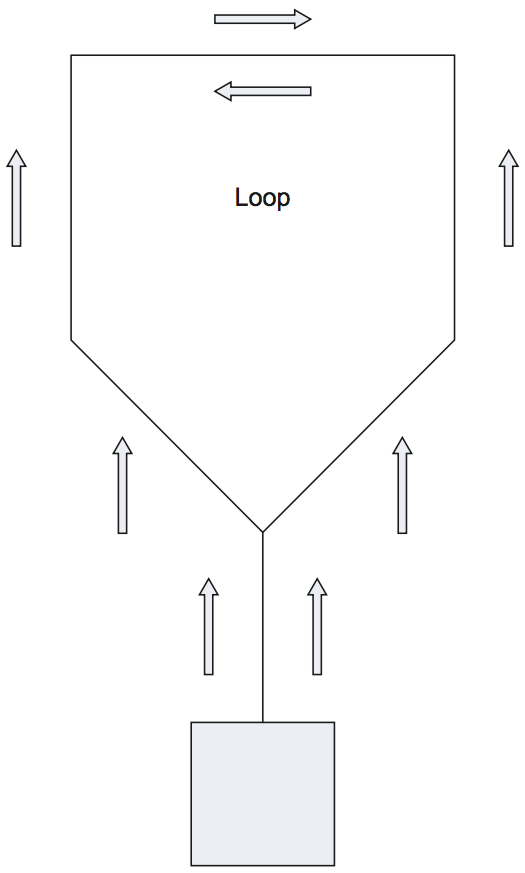
\includegraphics[scale=0.2, natwidth=525,natheight=873]{imgs/looptop.png}
  \caption{Looped topology}
}
\end{figure}
\newpage
Tale topologia è molto simile alla radial grid, ad eccezione del fatto che, a partire dalla sottostazione, i rami e le foglie hanno due cammini separati. L'obiettivo della looped topology è essere capace di resistere alle rotture interne alla rete, indipendentemente dal punto in cui si verificano; per questo motivo tale topologia risulta essere più costosa rispetto alla radial grid.
\newline \newline
Con il passare del tempo si è sentita sempre di più la necessità di svecchiare tali topologie, tenendo in conto tanti fattori e tante motivazioni.\newline
Considerando, per esempio, che quasi il 90\% dei guasti alla rete elettrica provengono dal sottosistema di distribuzione, le modifiche e i miglioramenti partono proprio da quest'ultimo. In più, il rapido aumento dei costi relativi ai combustibili fossili insieme all'inabilità delle aziende di espandere la loro potenza di generazione mantenendola in linea con la domanda sempre più crescente, ha accelerato il bisogno di modernizzare la rete di distribuzione introducendo tecnologie capaci di gestire meglio sia le richieste che i guadagni ottenuti. \newline
\begin{figure}[h]\centering{
  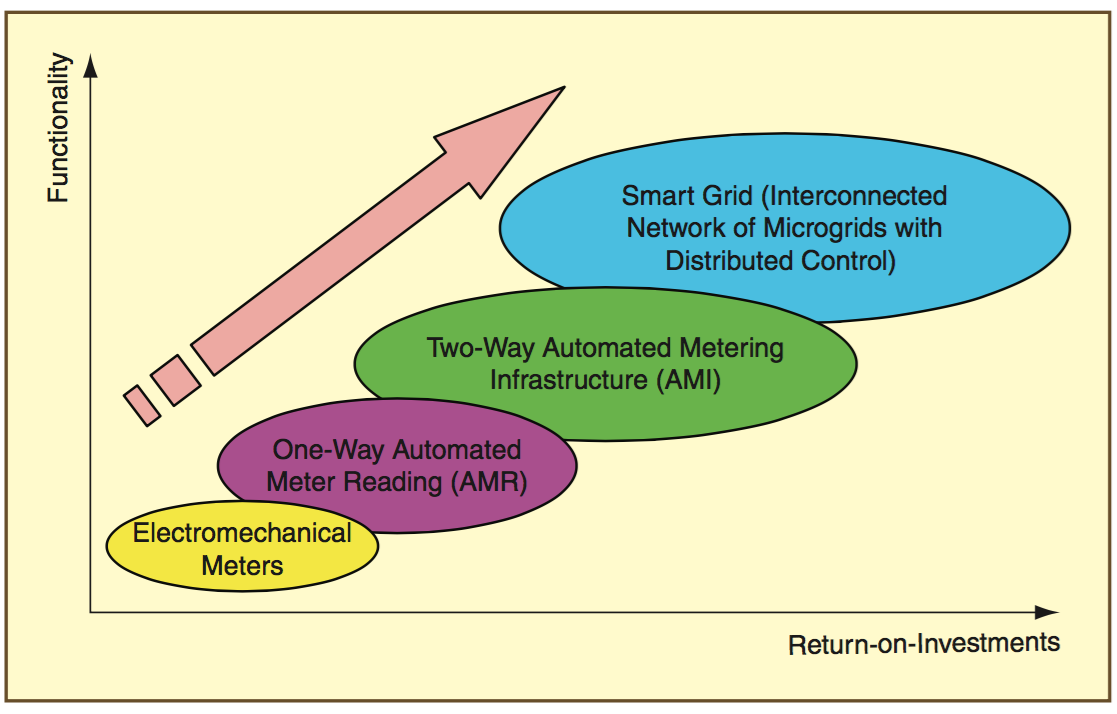
\includegraphics[scale=0.2, natwidth=1117,natheight=714]{imgs/evolution.png}
  \caption{L'evoluzione della smart grid}
}
\end{figure}

La figura 1.5 mostra che gli investimenti degli ultimi anni si sono focalizzati principalmente sull'aspetto della rete elettrica che riguarda le misurazioni (\textit{metering}). \newline I primi progetti in questo settore hanno visto la nascita dei sistemi di \textbf{automated meter reading} (AMR) all'interno del sistema di distribuzione. \newline
L'infrastruttura AMR (nata nel 1977) ha introdotto l'automazione nella rete elettrica. Attraverso una combinazione di tecnologie, incluse reti wireless e wired,   AMR ha permesso alle compagnie di leggere le misurazioni da remoto, di ottenere le informazioni quasi in real-time e di fornire agli utenti bollette basate sui consumi (in precedenza le compagnie emettevano le bollette basandosi sulle stime dei consumi del cliente).  \newline Inoltre, attraverso questo meccanismo di recupero informazioni tempestivo, le aziende sono state capaci di migliorare la produzione di energia attraverso un controllo più stretto durante periodi di alta e bassa richiesta. \newline \newline
Sebbene la teconologia AMR all'inizio abbia attirato molta attenzione, le aziende presto si sono rese conto che non risolve il loro problema principale: la gestione demand-side. A causa della sua comunicazione unidirezionale, le capacità di AMR sono ridotte alla sola lettura dei dati e non è permesso, per esempio, effettuare modifiche nel comportamento della rete a seconda delle informazioni ricevute. \newline Pertanto AMR ha avuto vita breve; le aziende, piuttosto che continuare ad investire su di essa, hanno preferito spostarsi verso l'\textbf{advanced metering infrastructure} (AMI). \newline
L'AMI (di cui si parlerà in dettaglio nel capitolo 2), è un'architettura che permette la comunicazione automatizzata e bidirezionale tra uno smart meter e una società di servizi. L'obiettivo è quello di fornire a tali società informazioni real-time circa i consumi energetici e permettere agli utenti di fare scelte informate sull'utilizzo dell'energia basate sui costi all'istante di utilizzo.
\newline
\newline
Il passo successivo nell'evoluzione della distribuzione della corrente elettrica è costituito dalla smart grid, che utilizza l'AMI come componente core per il recupero delle informazioni circa lo stato della rete e i consumi utente.
\newpage
\section{Perchè la Smart Grid}

\section{Cos'è una Smart Grid}

\section{Tecnologie coinvolte}